\chapter{Prospettiva Storica}

\section{Il Passato}

\paragraph{Nell'antichità:}

\begin{itemize}
  \item In Mesopotamia l'homo sapiens ha iniziato la sua età d'oro. 
  \item Circa 5000 anni fa nasce la scrittura. 
  \item Un'altra capacità che gli esseri umani sviluppano è quella di creare finzioni (storie, miti, patrie, religioni) allo scopo di aumentare la coesione tra di loro. I templi mesopotamici non erano così diversi dalle corporations moderne: avevano possedimenti, si occupavano di dare lavoro, etc. 
  \item Schiavitù nell'epoca romana: erano un oggetto, una proprietà. Se un nobile veniva ucciso da uno schiavo allora tutti gli altri schiavi dovevano venire giustiziati. 
  \item Commons: le parti di terra, mare, etc. non sono di una persona, ma della comunità.
  \item Facendo un salto avanti, nel 1968, Garret Hardin pubblica un libro in cui sostiene che i commons non  possono funzionare perché le risorse sono limitate (giustifica la proprietà privata). Una ventina di anni dopo Elinor Ostrom rispose che i sistemi di commons si autoregolano e quindi nessuno può approfittarne.
\end{itemize}

\paragraph{Dal feudalesimo:}

\begin{itemize}
  \item Gutenberg nel 1455 inventa la stampa a caratteri mobili. Viene usata per stampare la Bibbia, il ché porta alla diffusione della religione a prescindere dalla chiesa e poco dopo alla rivoluzione protestante di Lutero.
  \item I commons vengono dati a signori feudali sviluppando il latifondismo e aumentando la povertà degli abitanti dei villaggi. 
  \item Questo si ricollega a temi come l'espropriazione dei beni comuni (e.g. l'IA che fa concorrenza alle persone e viola il copyright).
  \item Non esistendo lo stato di diritto ogni feudatario si fa le sue regole.
  \item Nel '500 inizia la conquista delle Americhe. Si deve leggere un editto prima di assaltare i villaggi (questo è ripreso da aziende moderne come Google).
  \item A inizio del '600 Cartesio definisce il piano cartesiano (rendendo la geometria una questione di matematica). Oltre a questo sdogana il tabù relativo allo studio dei cadaveri. Il corpo, da entità sacra, diventa un qualcosa di studiabile. Introduce anche la visione del mondo come un grande orologio. Ma sostiene che linguaggio e ragionamento, in quanto dominio della mente e non del corpo, non sono studiabili.
  \item Successivamente, Julien Offray de La Mettrie, pubblica un trattato in cui parla di come la mente possa essere vista come una macchina modellabile. 
  \item Newton sfrutta l'idea di Cartesio e riconduce corpi celesti all'esperienza comune. Rendendo umano il divino. 
\end{itemize}

\section{La Rivoluzione Industriale e le sue Conseguenze}

\paragraph{La rivoluzione industriale:}

\begin{itemize}
  \item Adam Smith propose due teorie:
    \begin{itemize}
      \item Teoria della separazione dei lavori: persone specializzate fanno sempre la stessa cose. 
      \item La mano invisibile del mercato: elogio dell'imprenditoria.\footnote{Non è in grado di spiegarlo meglio perché è una stronzata.}
    \end{itemize}
  \item Tra la fine del '700 e l'inizio dell'800 nasce il \fancyglitter{luddismo}: un movimento di protesta operaia. 
  \item Il telaio ampio veniva utilizzato per il lavoro minorile, c'erano guerre in tutta europa, etc.
  \item Nel 1791 viene adottato il primo emendamento  che preveniva una serie di leggi. Il \fancyglitter{Panopticon} serve per sorvegliare potenzialmente tutti.
  \item 1833: New York Sun redatto da Benjamin Day. Costava meno, ma aveva la pubblicità all'interno. Era pieno di notizie scandalistiche, cronache giudiziarie, etc.
  \item 1860: Jules Cheret viene pagato per pubblicare manifesti pubblicitari. Dopo anni la popolazione di parigi si lamenta che questi manifesti rovinavano il panorama.
  \item 1890: viene pubblicizzata la Patent Medicine, generalmente truffe, verrà regolamentata nel 1906 con il Food and Drugs Act.
  \item 1893: Emile Durkheim mostra come la divisione dei lavori si sia spostata dalle fabbriche alla società. Si sono create dipendenze e coesioni tra le persone. Questo è un rischio perché nel momento in cui il padrone sostituirà i dipendenti con i robot questa mutua dipendenza si romperà.
  \item A fine '800 nasce il telefono come broadcast. Battaglia sui brevetti vinta da Bell. 
  \item Il telefono rimpiazza il telegrafo e crea un nuovo monopolio. 
  \item Nascita dei vari monopoli: treni, petrolio (Rockfeller), etc. 
  \item Herbert Spencer giustifica i monopoli con il \fancyglitter{darwinismo sociale}: il mercato ha le sue leggi per cui esistono vincitori e sconfitti. Punta a limitare la democrazia e sfocia nell'eugenetica.
  \item Sherman Act: tenta di limitare i monopoli. Nel 1911: azione antitrust che dissolve la standard oil. 
  \item Qualche anno dopo la Federal Trade Commission per regolare la concorrenza. 
  \item Theodore Vail: per le telecomunicazioni è utile avere un player che offra garanzie al pubblico. 
\end{itemize}

\paragraph{Le automobili:}

\begin{itemize}
  \item Inizialmente come bene di lusso. 
  \item Le strade però erano un bene comune, le auto erano pericolose. 
  \item Vengono obbligati i possessori di automobili a farle precedere da una persona con una bandiera rossa per segnalarne l'arrivo. 
  \item Viene fatta una grande campagna in cui venivano criticate le persone che vivevano per la strada. Viene creato il reato di camminamento in mezzo alla strada.
  \item Ford crea la produzione di massa delle automobili.
  \item Ai giorni nostri ci sono stati movimenti riguardo le piste ciclabili per reclamare la strada.
\end{itemize}

\begin{figure}[H]
    \centering
    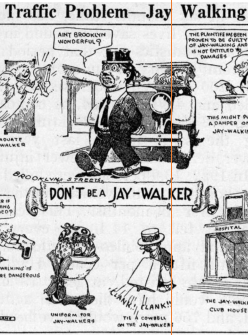
\includegraphics[scale=0.7]{02E/traffic.png}
    \caption{Reato di Jay-Walking.}
\end{figure}

\section{Verso il Mondo Moderno}

\paragraph{La modernità:}

\begin{itemize}
  \item 1908: Edison Motion Picture Patents, nasce il cinema. 
  \item Veniva bloccato l'import delle pellicole, il cinema era un monopolio. 
  \item 1912: Zukor crea la Paramount, dando vita al cinema statunitense. Si passa a un altro monopolio\footnote{Nothing ever happens, uh?}.
  \item Zio Sam: chiamata alle armi. La pubblicità viene usata a scopi propagandistici.
  \item Volontà di guerra, bisogna allinearsi alla volontà dello stato. 
  \item Contro la pubblicità si schiera Walter Lippmann mostrando come essa sia uno strumento di propaganda. 
  \item 1935: Riefenshal's Nazi Propaganda film. 
  \item La radio fu molto usata da Goebbels,  ministro della propaganda nella germania nazista.
  \item 1922: modello di servizio pubblico della BBC in UK. 
  \item Herbert Hoover: è inconcepibile che la radio possa inondare di pubblicità durante momenti privati.
  \item Questi problemi si trascinano fino ai giorni nostri con la pubblicità personalizzata nei feed\footnote{Esistono un sacco di adblocker o client customizzabili che bloccano la pubblicità.}. Tuttavia la pubblicità personalizzata viene scelta in base a cosa è conveniente per l'azienda.
  \item Theodore MacManus: inventa una strategia pubblicitaria che mette in luce le caratteristiche positive di un prodotto. 
  \item Nel 1923, Claude Hopkins crea una strategia più inquietante: utilizza la psicologia per creare pubblicità (demand engineering, branding, targeting).
  \item 1926: Coolidge, la pubblicità è l'anima del commercio. Lo stesso anno nasce un nuovo monopolio: NBC.
  \item 1927: Federal Radio Commission toglie la licenzia a centinaia di radio locali. 
  \item 1928: contenuto sponsorizzato, pagato dal brand che vuole fare la pubblicità. Ha parallelismi con la TV commerciale negli anni '80 in Italia in cui Silvio Berlusconi crea un consorzio di TV locali, compra le serie e i film che i piccoli emittenti non potevano permettersi, e manda a tutte le TV le videocassette con pubblicità.
  \item Sempre nel 1928, Edward Bernays inizia a pubblicizzare sigarette per le donne. Si inventa il termine le "Fiaccole della Libertà": modelle che andavano alle manifestazioni delle suffraggette fumando, allo scopo di vendere più sigarette.
  \item Nel 1936 in Germania, durante i giochi olimpici si diffonde la televisione. A dimostrazione che i monopoli frenano lo sviluppo invece di favorirlo. 
  \item Nl 1936 nasce anche l'audimeter per fare estrapolazioni statistiche su quello che piace alle persone. 
  \item 1939: la TV arriva in America dove copia la radio. 
  \item Un altro caso in cui i monopoli ostacolano il progresso è la questione AM vs. FM. 
  \item 1938: viene vietata la pubblicità ingannevole. 
  \item Nel 1939 inizia l'età dell'oro di Hollywood. Tuttavia in quegli anni dei cattolici, guidati da Daniel Lord impongono, mediante boicottaggio, degli standard di censura dei film.
\end{itemize}

\paragraph{I totalitarismi del '900:}

\begin{itemize}
  \item Già cominciato dalla fine della prima guerra mondiale. 
  \item I campi di lavoro erano in mano ai grandi monopolisti tedeschi. 
  \item Karl Polanyi si interroga sui fattori che hanno portato l'economia a favorire i monopoli e i monopoli a favorire un regime totalitario:
    \begin{itemize}
      \item Il mercato lasciato a sé stesso tende a diventare distruttivo. 
      \item Il capitalismo va contro le leggi prestabilite. 
      \item C'è bisogno di istituzioni autorevoli per fermarlo\footnote{Ho i miei dubbi che servano a qualcosa...}. 
      \item Le cose non vanno inevitabilmente in un'unica direzione, ma si viene convinti che sia così. Il mondo è una scelta fatta socialmente. 
    \end{itemize}
  \item Hannah Arendt capisce che le trasformazioni continuano ad avvenire continuamente: 
    \begin{itemize}
      \item La visione del capitalismo come ciclo che si ripete. 
      \item Soggiocazione del mondo naturale. 
      \item La natura del capitalismo è autodistruttiva, ha bisogno di un motore: ossia la costante mercificazione di aspetti della nostra vita. 
      \item L'imperialismo ha successo perché aggredisce aree non regolamentate\footnote{Come un certo qualcuno i cui genitori hanno delle miniere in sudafrica.}.
    \end{itemize}
  \item Nel 1913 nasce il comportamentamentismo in cui viene posto il problema di definire cos'è scienza. Si va a fare psicologia di ciò che è misurabile ossia il comportamento seguendo le teorie del condizionamento di Skinner (piccioni) e di Pavlov (cani). 
  \item La cosa prende campo anche in letteratura: 
    \begin{itemize}
      \item Aldous Huxley: Brave New World, società distopica in cui ogni persona è condizionata fin dalla nascita. La tecnologia è incompatibile con la libertà\footnote{Non sono totalmente d'accordo con questo. Ovvio che se sei uno schiavo di Microsoft o Apple è lapalissiano.}.
      \item George Orwell: 1984, mondo distopico in cui si è costantemente osservati. Tecnologia e libertà non sono compatibili...  
    \end{itemize}
\end{itemize}

\begin{figure}[H]
    \centering
    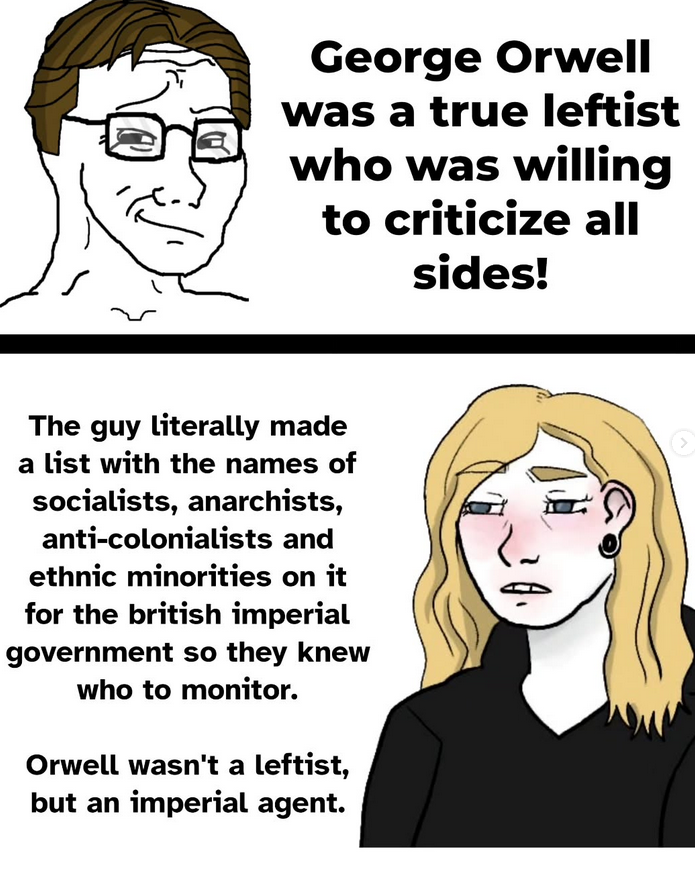
\includegraphics[scale=0.35]{02E/orwell.png}
    \caption{Per dare un po' più contesto su Orwell. Meme from @rizhomatic\_memer on IG.}
\end{figure}

\paragraph{Successivamente:}

\begin{itemize}
  \item Skinner: Walden 2, mondo idilliaco in cui viene presentato come bello il condizionamento della tecnologia\footnote{Idea ugualmente stupida come quelle di Huxley e Orwell.}. 
  \item Antitrust a Hollywood nel 1948.
  \item "Scoppia" la guerra fredda. Viene rafforzato il monopolio di AT\&T.
  \item Negli anni '50 Bork sostiene che i monopoli siano pericolosi solo se fanno male al consumatore. 
  \item Negli anni '70 si sviluppa l'idea del targeting. Robbin: si associano i territori a specifiche pubblicità creando clusters di consumatori. 
  \item Baran: invenzione del packet switch (che ha permesso la nascita di internet). 
  \item 1963: trasmissioni a lunga distanza di MCI. Intacca il monopolio. 
  \item 1969: antitrust contro IBM: produttore sia di hardware che software.
\end{itemize}








